\subsection{Extensiones del modelo}

El modelo del rotor rígido constituye una excelente primera aproximación para describir el movimiento rotacional de las moléculas diatómicas. Sin embargo, en la práctica las moléculas no son completamente rígidas: durante la rotación, las fuerzas centrífugas tienden a estirar el enlace, modificando ligeramente el momento de inercia y, por ende, las energías de los niveles rotacionales. Además, para moléculas no lineales, la rotación puede producirse alrededor de diferentes ejes principales, lo que origina diferentes tipos de rotores. En esta sección se presentan las extensiones más importantes al modelo básico.

\subsubsection*{Rotor no rígido y corrección centrífuga}

A medida que aumenta el número cuántico rotacional $J$, la velocidad angular de la molécula crece, generando una fuerza centrífuga que produce un alargamiento del enlace internuclear. Este fenómeno se traduce en una disminución del valor efectivo de la constante rotacional $B$, ya que el momento de inercia $I$ aumenta.  
Para tener en cuenta este efecto, se introduce la llamada \textbf{constante de distorsión centrífuga} $D$, y la expresión de los niveles de energía rotacional se corrige de la siguiente forma:

\[
E_J = B J(J+1) - D [J(J+1)]^2,
\]
donde el segundo término representa una pequeña corrección (del orden de $10^{-6}$ de $B$ en unidades típicas) que se vuelve significativa para valores altos de $J$.

El parámetro $D$ puede obtenerse experimentalmente a partir del análisis detallado de las posiciones de las líneas rotacionales observadas. El espaciado entre líneas ya no es exactamente constante, sino que disminuye ligeramente con $J$:
\[
\nu = 2B(J+1) - 4D(J+1)^3.
\]
Esta dependencia cúbica permite ajustar los datos experimentales y determinar tanto $B$ como $D$ con gran precisión \cite[p.~218]{bernath2016spectra}.  
De este modo, la espectroscopía de microondas no solo proporciona las distancias de enlace, sino también información sobre la \textbf{flexibilidad de los enlaces químicos} y la \textbf{energía vibracional acoplada} al movimiento rotacional.

\subsubsection*{Moléculas no lineales y tipos de rotores}

Cuando una molécula presenta más de dos átomos, la rotación puede ocurrir alrededor de varios ejes, definidos por los \textbf{momentos principales de inercia} $I_A$, $I_B$ e $I_C$. Según las relaciones entre ellos, se distinguen tres tipos fundamentales de rotores:

\begin{itemize}
    \item \textbf{Rotor lineal:} posee un único eje de rotación (como CO$_2$ o HCN), con dos momentos de inercia iguales y uno nulo. Su espectro sigue la misma forma que el de una molécula diatómica.
    \item \textbf{Rotor simétrico:} cumple $I_A = I_B \neq I_C$ (prolato) o $I_A \neq I_B = I_C$ (oblato). Ejemplos típicos son CH$_3$Cl (prolato) y BF$_3$ (oblato). En estos casos, la estructura del espectro rotacional depende de la proyección del momento angular sobre el eje de simetría.
    \item \textbf{Rotor asimétrico:} todos los momentos de inercia son diferentes ($I_A \neq I_B \neq I_C$), como en el caso del vapor de agua (H$_2$O). Su espectro rotacional es más complejo y requiere tratamiento numérico.
\end{itemize}

El estudio de estos sistemas permite determinar con precisión las \textbf{geometrías tridimensionales moleculares} y las simetrías internas, constituyendo un campo fundamental en la física molecular y la astroquímica.

\subsubsection*{Transiciones hiperfinas e isótopos}

Además de los efectos rotacionales y centrífugos, algunos espectros de microondas presentan una estructura aún más fina debido a la \textbf{interacción hiperfina}, producida por el acoplamiento del momento magnético nuclear con el campo magnético generado por el movimiento electrónico. Esta interacción produce pequeños desdoblamientos de las líneas rotacionales, típicamente del orden de los kHz a MHz.

Por otro lado, la sustitución isotópica (por ejemplo, HCl $\rightarrow$ DCl o $^{12}$CO $\rightarrow$ $^{13}$CO) modifica la masa reducida $\mu$, y por tanto el momento de inercia $I = \mu r^2$. Como consecuencia, el valor de la constante rotacional $B$ cambia de forma predecible:
\[
B \propto \frac{1}{\mu}.
\]
Este hecho permite identificar distintos isótopos moleculares mediante el desplazamiento de las frecuencias de las líneas rotacionales, lo cual es de gran utilidad en estudios astrofísicos y en la caracterización precisa de compuestos químicos \cite[p.~145]{hollas2004modern}.



\begin{figure}[H]
\centering
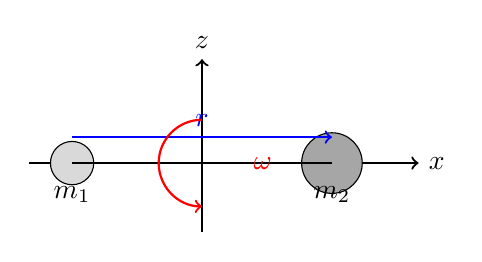
\begin{tikzpicture}[scale=1.1]
% Eje
\draw[thick, ->] (-2,0) -- (2.5,0) node[right] {$x$};
\draw[thick, ->] (0,-0.8) -- (0,1.2) node[above] {$z$};

% Átomos
\filldraw[fill=gray!30] (-1.5,0) circle (0.25) node[below=5pt] {$m_1$};
\filldraw[fill=gray!70] (1.5,0) circle (0.35) node[below=5pt] {$m_2$};

% Enlace
\draw[thick] (-1.5,0) -- (1.5,0);

% Vector r
\draw[thick, ->, blue] (-1.5,0.3) -- (1.5,0.3) node[midway, above, blue] {$r$};

% Rotación
\draw[->, red, thick] (0,0.5) arc[start angle=90, end angle=270, radius=0.5];
\node[red] at (0.7,0) {$\omega$};
\end{tikzpicture}
\caption{Rotor lineal: la molécula rota perpendicularmente al eje del enlace. Ejemplo: HCl, CO.}
\end{figure}

\begin{figure}[H]
\centering
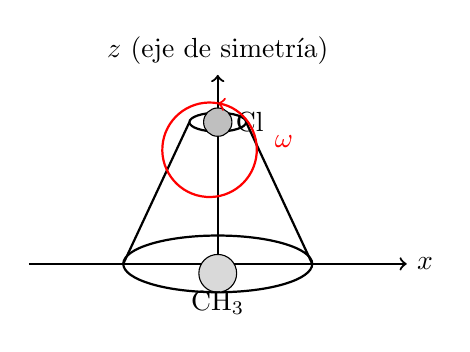
\begin{tikzpicture}[scale=1.2]
% Ejes
\draw[->, thick] (0,0) -- (0,2) node[above] {$z$ (eje de simetría)};
\draw[->, thick] (-2,0) -- (2,0) node[right] {$x$};

% Molécula (cono)
\draw[thick] (0,0) ellipse (1 and 0.3);
\draw[thick] (0,1.5) ellipse (0.3 and 0.1);
\draw[thick] (-1,0) -- (-0.3,1.5);
\draw[thick] (1,0) -- (0.3,1.5);

% Átomo central
\filldraw[fill=gray!50] (0,1.5) circle (0.15) node[right=3pt] {Cl};

% Grupo CH3
\filldraw[fill=gray!30] (0,-0.1) circle (0.2);
\node[below=3pt] at (0,-0.1) {CH$_3$};

% Eje rotación
\draw[->, red, thick] (0,1.7) arc[start angle=80, end angle=440, radius=0.5];
\node[red] at (0.7,1.3) {$\omega$};
\end{tikzpicture}
\caption{Rotor simétrico prolato: ejemplo de molécula CH$_3$Cl con eje de simetría principal.}
\end{figure}

\begin{figure}[H]
\centering
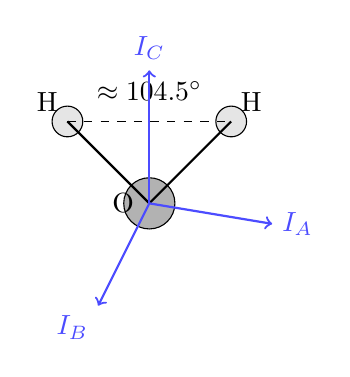
\begin{tikzpicture}[scale=1.3]
% Oxígeno
\filldraw[fill=gray!60] (0,0) circle (0.25) node[left=2pt] {O};

% Hidrógenos
\filldraw[fill=gray!20] (-0.8,0.8) circle (0.15) node[above left] {H};
\filldraw[fill=gray!20] (0.8,0.8) circle (0.15) node[above right] {H};

% Enlaces
\draw[thick] (0,0) -- (-0.8,0.8);
\draw[thick] (0,0) -- (0.8,0.8);

% Ángulos
\draw[dashed] (-0.8,0.8) -- (0.8,0.8);
\node at (0,1.1) {$\approx 104.5^\circ$};

% Ejes principales (I_A, I_B, I_C)
\draw[->, blue!70, thick] (0,0) -- (1.2,-0.2) node[right] {$I_A$};
\draw[->, blue!70, thick] (0,0) -- (-0.5,-1.0) node[below left] {$I_B$};
\draw[->, blue!70, thick] (0,0) -- (0,1.3) node[above] {$I_C$};
\end{tikzpicture}
\caption{Rotor asimétrico: molécula de agua (H$_2$O) con tres momentos de inercia distintos.}
\end{figure}


\begin{figure}[H]
\centering
\begin{tikzpicture}[scale=1.1]
% Niveles de energía
\foreach \y/\J in {0/0,1.5/1,3.2/2,5.2/3} {
    \draw[thick] (0,\y) -- (2.5,\y);
    \node[left] at (0,\y) {$J=\J$};
}

% Transiciones principales
\foreach \y in {0.75,2.3,4.2} {
    \draw[->, red, thick] (2.5,\y) -- (4.5,\y+0.75);
}

% Desdoblamiento isotópico
\foreach \y in {0.1,1.6,3.4,5.3} {
    \draw[thick, blue, opacity=0.6] (5.5,\y) -- (8,\y);
}

\node[red] at (3.5,5.2) {$\Delta J = +1$};
\node[blue] at (6.8,5.8) {Desplazamiento isotópico};

\end{tikzpicture}
\caption{Esquema del espectro rotacional mostrando transiciones $\Delta J=+1$ y desplazamientos isotópicos o hiperfinos.}
\end{figure}





